\newpage
\section{Discussion}
% \begin{itemize}
%     \item What is new?
%     \item What is as expected? What is unexpected? 
%     \item How exact are the results? Which assumptions did I make?
%     \item Which things have I left out? What can be investigated further?
%     \item How can one measure/test the findings?
% \end{itemize}

\begin{figure}[H]
    \centering
    \subfigure[Spinstructure for SC with RKKY $J= 2$ (no SOC) ]{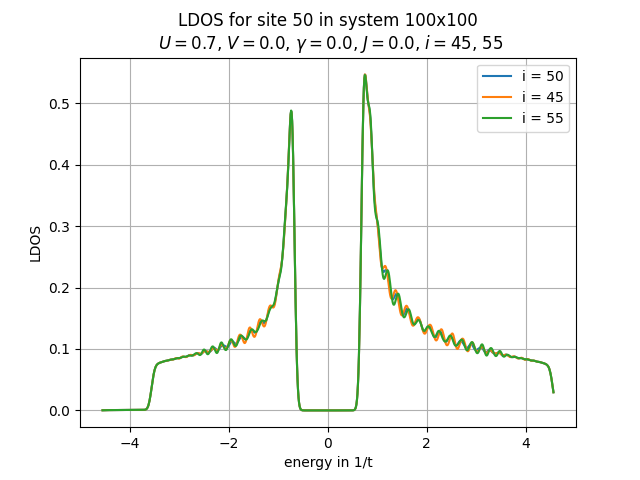
\includegraphics[width=0.48\textwidth]{Images/ldos_tri_100_100_0.5_0.7_0.0_0.0_0.0_45_55.png}}
    \subfigure[Spinstructure for SC with RKKY $J=5$ (no SOC)]{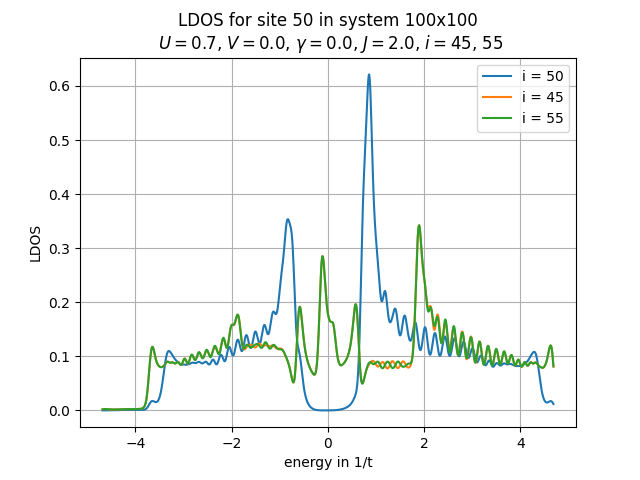
\includegraphics[width=0.48\textwidth]{Images/ldos_tri_100_100_0.5_0.7_0.0_0.0_2.0_45_55.png}}
    \caption{bands are splitting}
    \label{fig:spinstruct_soc_rkkyComp}
\end{figure}

\begin{figure}[H]
    \centering
    \subfigure[Spinstructure for SC with RKKY $J= 2$, with SOC ]{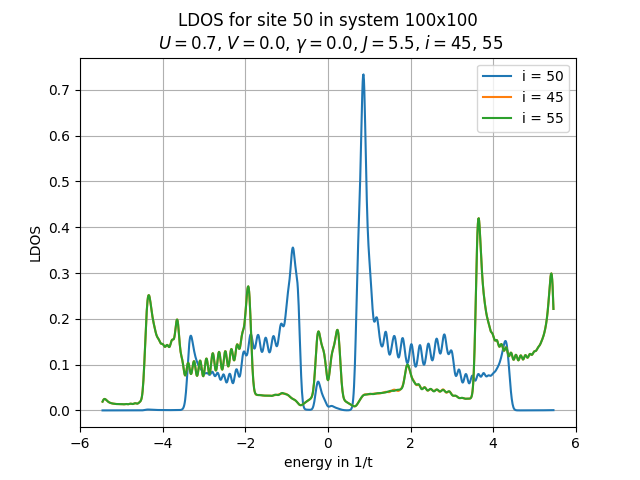
\includegraphics[width=0.48\textwidth]{Images/ldos_tri_100_100_0.5_0.7_0.0_0.0_5.5_45_55.png}}
    \subfigure[40x40, mu=0.5, U=0.5, V=1.2, gamma=0.15, J=2, i=15,25; \newline t=1, U=0.1, V=0.4, gamma=0.2, J=0.3, mu=0.5, N=10, i=3,6]{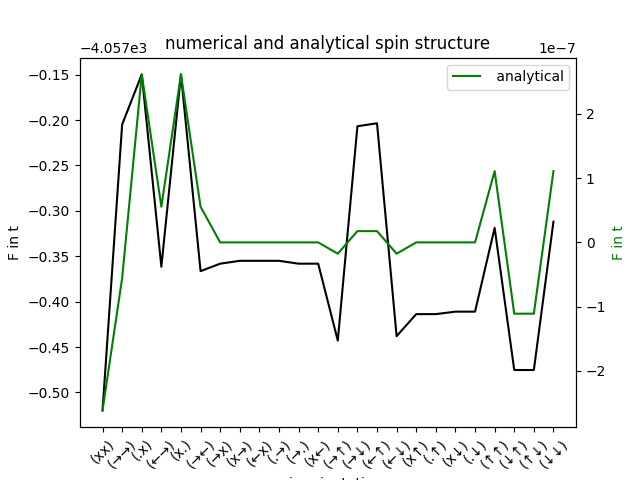
\includegraphics[width=0.48\textwidth]{Images/spinstructure_comparison.png}}
    \caption{bands do not overlap any longer; analytical vs. numerical result}
    \label{fig:spinstruct_sc+soc_rkkyComp}
\end{figure}

\begin{figure}[H]
    \centering
    \subfigure[Spinstructure for SC with RKKY $J= 2$ (no SOC) ]{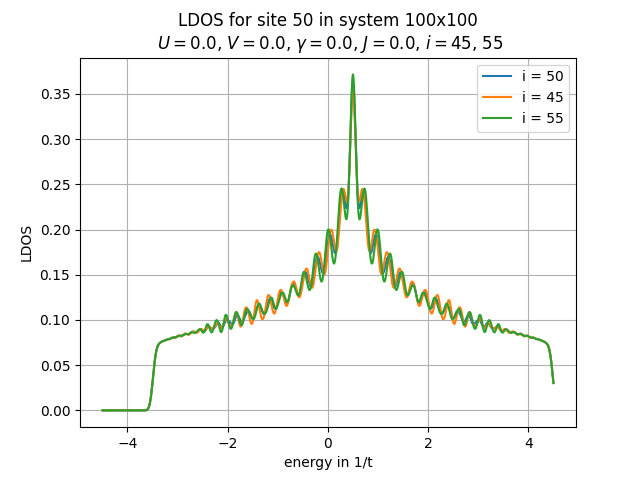
\includegraphics[width=0.48\textwidth]{Images/ldos_tri_100_100_0.5_0.0_0.0_0.0_0.0_45_55.png}}
    \subfigure[Spinstructure for SC with RKKY $J=5$ (no SOC)]{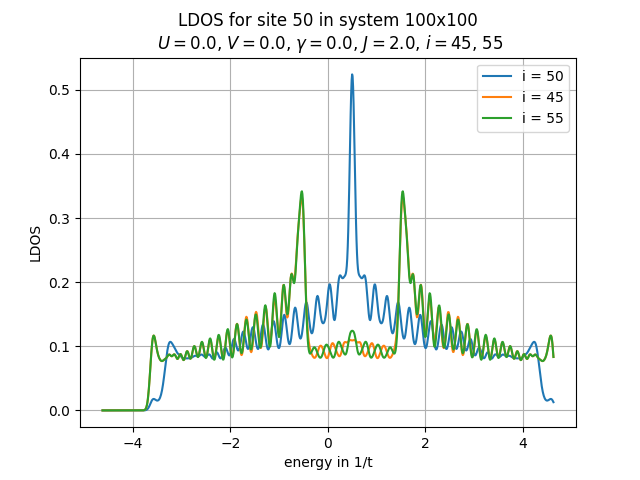
\includegraphics[width=0.48\textwidth]{Images/ldos_tri_100_100_0.5_0.0_0.0_0.0_2.0_45_55.png}}
    \caption{bands are splitting}
    \label{fig:spinstruct_soc_rkkyComp}
\end{figure}

\begin{figure}[H]
    \centering
    \subfigure[Spinstructure for SC with RKKY $J= 2$, with SOC ]{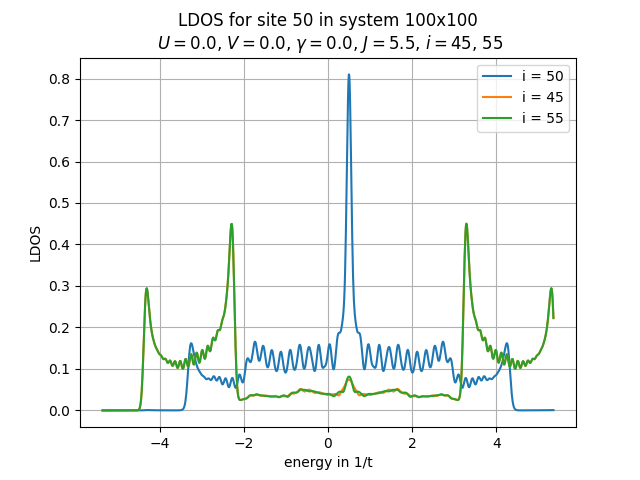
\includegraphics[width=0.48\textwidth]{Images/ldos_tri_100_100_0.5_0.0_0.0_0.0_5.5_45_55.png}}
    % \subfigure[40x40, mu=0.5, U=0.5, V=1.2, gamma=0.15, J=2, i=15,25; \newline t=1, U=0.1, V=0.4, gamma=0.2, J=0.3, mu=0.5, N=10, i=3,6]{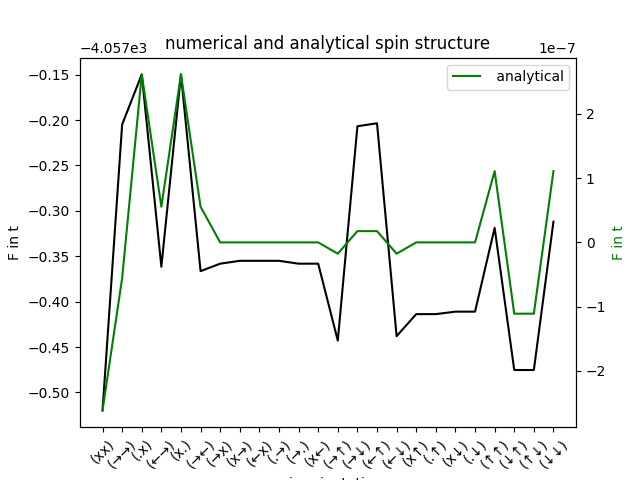
\includegraphics[width=0.48\textwidth]{Images/spinstructure_comparison.png}}
    \caption{bands do not overlap any longer; analytical vs. numerical result}
    \label{fig:spinstruct_sc+soc_rkkyComp}
\end{figure}

% \subsection{Ideas from Atousa's work}
% \subsubsection{Check if superconducting}
% compare free energy of normal state and compare if superconducting state has lower free energy - really necessary? SC is not spin-split like Atousa's \newline
% $\Rightarrow$ free energy of superconducting system is significantly lower than normal metal system, so it is indeed superconducting
% \subsubsection{Experiments}
% she has an entire section on experimental realization, so maybe I can learn something from that